\documentclass{standalone}
\usepackage{tikz}
\usepackage{amsmath}

\begin{document}

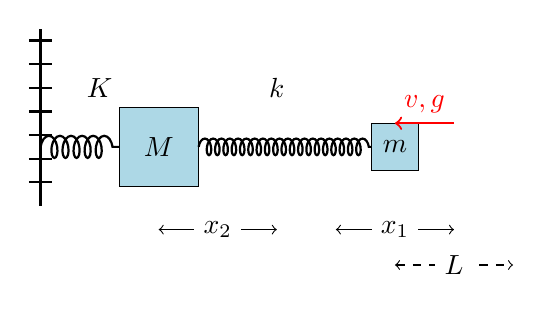
\begin{tikzpicture}[scale=1.5]
    % Colors
    \definecolor{masscolor}{RGB}{173, 216, 230} % Light blue

    % Wall
    \draw[thick] (-1,0) -- (-1,1.5);
    \foreach \y in {0.2,0.4,...,1.4}
        \draw[thick] (-1.1,\y) -- (-0.9,\y);

    % Mass M
    \node[draw, fill=masscolor, minimum width=1cm, minimum height=1cm] (M) at (0,0.5) {$M$};

    % Mass m
    \node[draw, fill=masscolor, minimum width=0.6cm, minimum height=0.6cm] (m) at (2,0.5) {$m$};

    % Springs
    \draw[thick, decorate, decoration={coil, aspect=0.5, segment length=4pt, amplitude=4pt}] (-1,0.5) -- (M.west);
    \draw[thick, decorate, decoration={coil, aspect=0.5, segment length=3pt, amplitude=3pt}] (M.east) -- (m.west);

    % Labels for springs
    \node at (-0.5,1) {$K$};
    \node at (1,1) {$k$};

    % Distances
    \draw[<->] (0,-0.2) -- node[fill=white] {$x_2$} (1,-0.2);
    \draw[<->] (1.5,-0.2) -- node[fill=white] {$x_1$} (2.5,-0.2);
    \draw[<->, dashed] (2,-0.5) -- node[fill=white] {$L$} (3,-0.5);

    % Forces
    \draw[->, red, thick] (2.5,0.7) -- ++(-0.5,0) node[midway, above, sloped] {$v, g$};

\end{tikzpicture}

\end{document}